%% Part of Stellarium User Guide 0.15+
%% History:
%% 2016-04-17 New chapter.
%% 2025-02-17: Rewrite for new SC format


\chapter{Adding Sky Cultures}
\label{ch:SkyCultures}
\chapterauthor*{Georg Zotti, with additions by Alexander Wolf and Susanne M. Hoffmann}


Stellarium comes with a nice set of sky cultures from all
over the world (see section~\ref{sec:gui:view:skyculture}). For ethnographers or
historians of science it may be a worthwhile consideration to
illustrate the sky culture of the people they are studying. It is not
very hard to do so, but depending on your data, may require some
skills in image processing.

Version 25.1 introduces a completely new format for skyculture data.\newFeature{25.1} 
If you are interested in the old format, please refer to the 24.4 edition of the User Guide.
In case you have created your own skycultures, we have created a format converter  described in section~\ref{ch:SkyCultures:converter}.


If you add a new sky culture, please adhere to this description for an optimal result!
Some features regarding translation and multilinguality have evolved
over the years, and not all sky cultures currently included in
Stellarium adhere to the standards described in the following
sections. Incomplete skycultures may be improved, or removed when found too deficient.



A \indexterm{sky culture} in Stellarium is the entity that consists of 
\begin{itemize}
\item a description of the role these constellations and other celestial features (clouds, polar lights (aurorae), meteors, comets, \ldots) 
      had or still have for the human culture that used or use these constellations, including some relevant background on the culture.
\item a set of names for constellations 
\item stick figure definitions connecting stars into those constellations
\item (optional) a list of names for individual stars
\item (optional) artwork supporting the stick figures
\item (optional) a description of boundaries or borders between the constellations
\item (optional) names and stick figure definitions of additional figures of lesser importance, termed \indexterm{asterisms}.
\item A CC-licence that the author of the SC chooses; this is valid for the entire set of files, i.e. all texts and images provided.
\end{itemize}




\iffalse


You can take the \file{inuit} directory as template to start with. Just copy the folder 
\file{C:\textbackslash{}Program Files\textbackslash{}Stellarium\textbackslash{}skycultures\textbackslash{}inuit} to
\file{C:\textbackslash{}Users\textbackslash{}[YOU]\textbackslash{}AppData\textbackslash{}Roaming\textbackslash{}Stellarium\textbackslash{} skycultures\textbackslash{}myculture}

In the folder you see image files for the constellation artwork, and all
other files with various extensions are text files. 
\fi


\section{Text description}
\label{sec:skycultures:description}
\label{SC:description.md}


A sky culture must contain the file \file{description.md}, this is a text in \program{Markdown} format. 
Markdown is a plaintext format which allows the simple declaration of text regions like sections, subsections, lists, images, or references. 
The file is automatically broken into pieces, translated and converted to HTML for display. Also some important skyculture components are extracted from here.

The first line of the file starts with the only Level 1 header, 
i.e., a line starting with a single hash (\texttt{\#}), 
a space and then the \emph{name} of the skyculture. 
This name is used in the selection list in the Sky Culture GUI (see \ref{sec:gui:view:skyculture}). 
 
The other sections typically start with Level 2 or 3 headers (with two or three hash characters) which are displayed as smaller section and 
subsection titles (HTML: \texttt{h2} or \texttt{h3}, respectively).  

The continuous text should be formatted like that, please do not add newlines where they do not signal the end of a paragraph with an empty line. 
Use an editor which just auto-wraps long lines to the window width. 
These long lines/paragraphs are automatically fed into the translation system. References (see \ref{SC:references}) should be given like \texttt{[\#42]}.
 
You can also have embedded images in the file (your book cover?
Views of sacred landscapes/buildings/artwork/\ldots?), just provide them in 
PNG or JPG format please. 

You should provide a good description in the interest of future users:
some cultural/ethnographical background of the users of this sky culture,
history of sky culture research that provided this work, tables of names/translations,
links to external resources, whatever seems suitable.  The length of the description texts is not limited.

The skyculture description should include the following Level 2 sections. Any other section must be a subsection (i.e. Level 3 or deeper) of one of these sections. Each of these sections will have its own entry in the translations files.

\begin{description}
\item \texttt{Introduction} -- a summary that could ideally be shown on a small screen entirely.
\item \texttt{Description} -- the actual text of the description.
\item \texttt{Constellations} -- a sequence of Level 5 sections, where the header names a constellation, and the contents gives some information on it.
\item \texttt{References} -- a list of references, see \ref{SC:references} for details.
\item \texttt{Authors} -- all authors and acknowledgments go here.
\item \texttt{License} -- either a license id (see \ref{SC:license}), or a sequence of lines separated by empty lines (i.e. Markdown paragraphs) describing which part of the culture has which license, in the format "Sky culture item: License-ID".
\end{description}

To allow the correct display of special characters like ÄÖÜßáé you must provide the file in UTF-8 encoding. 
If you write only English/ASCII, this may not be relevant.


\subsection{References}
\label{sec:skycultures:references}
\label{SC:references}

The optional Level 2 section ``References'' contains a list of information sources. 
Each line of the section contains one record of 2 discernible fields: 
a hyphen followed by a numerical key in brackets, 
a colon and then the actual description of the reference. The latter may include hyperlinks,
 e.g.:

\begin{configfile}[\scriptsize]
 - [#1]: Kunitzsch, P.; Smart T. (2006). "A Dictionary of Modern star Names: ...
\end{configfile}

This list is most important for ``traditional'' sky cultures collected from various sources to provide traceable references. 

\paragraph{Caution!} These reference numbers are not only used in the text, but also in the data description. If you re-arrange references, 
you must also fix all affected references in the JSON file (\ref{SC:index.json}).


\subsection{License}
\label{sec:skycultures:licenses}
\label{SC:license}

The level 2 section ``License''  is mandatory if you want your sky culture to be distributed with
Stellarium to prevent ``unexpected'' distribution of your content to other
software or applications out of our hands.  
\iffalse
The license info will be decoded for human readable hints about allowed permissions for sky culture in the GUI.
\fi

We recommend to use one of the following possible licenses in this section: 
\begin{description}
  \item[GNU GPL v2.0 (or later)] -- this is the most famous ``copyleft'' license for code and it may be acceptable also for text and data.
  \item[CC0] (No Rights Reserved) -- this is a ``don't care'' license. Content may be freely distributed without attribution for all purposes. 
  \item[CC BY] (Creative Commons Attribution License) -- this license lets others distribute, remix, adapt, and build upon your work, even commercially, 
    as long as they credit you for the original creation.
    This is the most accommodating of licenses offered. Recommended for maximum dissemination and use of licensed materials.
  \item[CC BY-SA] (Creative Commons Attribution-ShareAlike License) -- this license lets others remix, adapt, and build upon your work even for commercial purposes, 
    as long as they credit you and license their new creations under the identical terms.
    This license is often compared to ``copyleft'' free and open source software licenses. 
	All new works based on yours will carry the same license, so any derivatives will also allow commercial use.
    This is the license used by Wikipedia, and is recommended for materials that would benefit from incorporating content from Wikipedia and similarly licensed projects.
  \item[CC BY-ND] (Creative Commons Attribution-NoDerivatives License) -- this license lets others reuse the work for any purpose, including commercially; 
    however, it cannot be shared with others in adapted form, and credit must be provided to you.
  \item[CC BY-NC] (Creative Commons Attribution-NonCommercial License) -- this license lets others remix, adapt, and build upon your work non-commercially, 
    and although their new works must also acknowledge you and be non-commercial, they don’t have to license their derivative works on the same terms.
  \item[CC BY-NC-SA] (Creative Commons Attribution-NonCommercial-ShareAlike License) -- this license lets others remix, adapt, and build upon your work non-commercially, 
    as long as they credit you and license their new creations under the identical terms.
  \item[CC BY-NC-ND] (Creative Commons Attribution-NonCommercial-NoDerivatives License) -- this license is the most restrictive of the six main Creative Commons licenses, 
    only allowing others to download your works and share them with others as long as they credit you, but they can’t change them in any way or use them commercially.
  \item[FAL] For illustrations we also expect usage of the \textbf{Free Art License}\footnote{\url{https://artlibre.org/licence/lal/en/}} (in addition to any other licenses) --
    it is a ``copyleft'' license that grants the right to freely copy, distribute, and transform creative works. You can specify, e.g., ``GPL2, FAL'' to 
	indicate that the images are additionally released under Free Art License.
\end{description}

\noindent Creative Commons provides a range of licenses\footnote{Creative
  Commons License Chooser --
  \url{https://creativecommons.org/choose/}}, each of which grants
different rights to use the materials licensed under them. All of
these licenses offer more permissions than ``all rights
reserved''. Some of Creative Commons are free and some are
non-free. For example you can apply only the most permissive of its
licenses (\textbf{CC0}, \textbf{CC BY} and \textbf{CC BY-SA}) to
material you create, to meets the Freedom Defined definition of a
``Free Cultural Work''.\footnote{See Creative Commons website to
  details --
  \url{https://creativecommons.org/share-your-work/public-domain/freeworks}}

If you have used one of the keys above in your \texttt{license} entry,
a short (unofficial!  Informative only) description of license
conditions will be displayed. You can use other licenses as well, but
then please describe the conditions sufficiently well in this section.


\paragraph{Caution for users!} While Stellarium is provided under the free GPL v2.0 licence which allows for commercial use,
some of our sky cultures have been contributed under CC NC/ND licenses,
i.e., are for noncommercial use only.  Please respect their heritage
holders and check the CC licence version in the description before
you use sky cultures in public events like TV documentaries, YouTube
videos, lectures, planetarium shows or printed matter. If in doubt,
contact the respective authors.



%%%%%%%%%%%%%%%%%%%%%%%%%%%%%%%%%%%%%%%%%%%%%%%%%%%%%%%%%%%%%%%%%%%%%%%%%%%%%%%%%%%%%%%%%%%%%%%%%%%%%%%%%%%%%%%%%%%%%%%%%%%%%%%%%%%%%%%%%%%%%%%%%%%%

\section{Technical data: index.json}
\label{sec:skycultures:index.json}
\label{SC:index.json}

%% JSON tag. (tag exists)
\newcommand{\jtag}[1]{\texttt{"#1"}}


The file \file{index.json} contains all ``technical data'' of the skyculture. 
JSON is a text-based format in which strings, numerical values and arrays can be stored in nested \emph{dictionaries}, 
i.e. unordered collections of comma-separated \texttt{"tag": value} pairs in braces: \texttt{\{ "Tag1": "Value1", "number": 123.456 \}}. 
Values can be strings, numbers, arrays or other dictionaries. Arrays are ordered sequences in \texttt{[...]} delimiters.  
You must take care to close any open brackets and separate entries by commas. 


\begin{jsonfile}[\scriptsize]
{
  "id": "modern",
  "region": "World",
  "classification": ["traditional"],
  "fallback_to_international_names": false,
  "asterisms": [ ... ],
  "constellations": [ ... ],
  "edges_type": "iau",
  "edges_source": "https://pbarbier.com/constellations/edges_18.txt",
  "edges_epoch": "B1875",
  "edges": [ ... ],
  "common_names": { ... }
}
\end{jsonfile}

in which
\begin{description}
\item[\jtag{id}] A unique identifier for program-internal use. It is never displayed to users. 
\item[\jtag{region}] See \ref{SC:region}
\item[\jtag{classification}] See \ref{SC:classification}
\item[\jtag{fallback\_to\_international\_names}] if \texttt{true}, the IAU-approved star names are loaded after all names given here, 
so names will be mixed without a clear separation, and newly-approved star names will just appear automatically. 
Also all DSO names from \file{nebulae/default/names.dat} are loaded.
This is most useful for skycultures which have no names of their own, or where such mix is intended, 
like \jtag{personal} contemporary skycultures (see ~\ref{SC:classification}) which are allowed to auto-adapt to newly given names. 
% These are used by a related project. We can safely ignore them.
%\item[\jtag{thumbnail}] ignored
%\item[\jtag{thumbnail\_bscale}] ignored
%\item[\jtag{highlight}] ignored
\item[\jtag{common\_names}] includes names for star, planet and deep-sky objects, see \ref{SC:common_names}
\item[\jtag{constellations}] describes constellations, see \ref{SC:constellations}
\item[\jtag{edges\ldots}] describes boundaries between constellations, see \ref{SC:boundaries}
\item[\jtag{asterisms}]  describes asterisms, see \ref{SC:asterisms}
\end{description}

Tags not described here may be used in other programs but are ignored by Stellarium.

\subsection{Region}
\label{sec:skycultures:region}
\label{SC:region}

The ``region'' tag marks the origin region of the respective sky culture.
It allows some form of additional grouping. The names of regions are following the United Nations
geoscheme UN~M49\footnote{Standard country or area codes for statistical use (M49) -- \url{https://unstats.un.org/unsd/methodology/m49/}}:
\begin{description}
	\item[Northern Africa] -- Algeria, Egypt, Libya, Morocco, Sudan, Tunisia, Western Sahara.
	\item[Eastern Africa] -- British Indian Ocean Territory, Burundi, Comoros, Djibouti, Eritrea, Ethiopia, French Southern Territories, Kenya,
          Madagascar, Malawi, Mauritius, Mayotte, Mozambique, Réunion, Rwanda, Seychelles, Somalia, South Sudan, Uganda, United Republic of Tanzania, Zambia, Zimbabwe.
	\item[Central Africa] -- Angola, Cameroon, Central African Republic, Chad, Congo, Democratic Republic of the Congo, Equatorial Guinea, Gabon, Sao Tome and Principe.
	\item[Southern Africa] -- Botswana, Eswatini, Lesotho, Namibia, South Africa.
	\item[Western Africa] -- Benin, Burkina Faso, Cabo Verde, Côte d’Ivoire, Gambia, Ghana, Guinea, Guinea-Bissau, Liberia,
          Mali, Mauritania, Niger, Nigeria, Saint Helena, Senegal, Sierra Leone, Togo.
	\item[Caribbean] -- Anguilla, Antigua and Barbuda, Aruba, Bahamas, Barbados, Bonaire, Sint Eustatius and Saba, British Virgin Islands,
          Cayman Islands, Cuba, Curaçao, Dominica, Dominican Republic, Grenada, Guadeloupe, Haiti, Jamaica, Martinique, Montserrat, Puerto Rico, Saint Barthélemy,
          Saint Kitts and Nevis, Saint Lucia, Saint Martin (French Part), Saint Vincent and the Grenadines, Sint Maarten (Dutch part),
          Trinidad and Tobago, Turks and Caicos Islands, United States Virgin Islands.
	\item[Central America] -- Belize, Costa Rica, El Salvador, Guatemala, Honduras, Mexico, Nicaragua, Panama.
	\item[Southern America] -- Argentina, Bolivia (Plurinational State of), Bouvet Island, Brazil, Chile, Colombia, Ecuador,
          Falkland Islands (Malvinas), French Guiana, Guyana, Paraguay, Peru, South Georgia and the South Sandwich Islands, Suriname,
          Uruguay, Venezuela (Bolivarian Republic of).
	\item[Northern America] -- Bermuda, Canada, Greenland, Saint Pierre and Miquelon, United States of America.
	\item[Antarctica] -- Antarctica.
	\item[Northern Asia] -- Russian Federation (Asian part).
	\item[Central Asia] -- Kazakhstan, Kyrgyzstan, Tajikistan, Turkmenistan, Uzbekistan.
	\item[Eastern Asia] -- China, Hong Kong Special Administrative Region of China, Macao Special Administrative Region of China,
          Democratic People's Republic of Korea, Japan, Mongolia, Republic of Korea, Taiwan.
	\item[South-eastern Asia] -- Brunei Darussalam, Cambodia, Indonesia, Lao People's Democratic Republic, Malaysia, Myanmar,
          Philippines, Singapore, Thailand, Timor-Leste, Viet Nam.
	\item[Southern Asia] -- Afghanistan, Bangladesh, Bhutan, India, Iran (Islamic Republic of), Maldives, Nepal, Pakistan, Sri Lanka.
	\item[Western Asia] -- Armenia, Azerbaijan, Bahrain, Cyprus, Georgia, Iraq, Israel, Jordan, Kuwait, Lebanon, Oman, Qatar,
          Saudi Arabia, State of Palestine, Syrian Arab Republic, Türkiye, United Arab Emirates, Yemen.
	\item[Eastern Europe] -- Belarus, Bulgaria, Czechia, Hungary, Poland, Republic of Moldova, Romania, Russian Federation (European part), Slovakia, Ukraine.
	\item[Northern Europe] -- Åland Islands, Channel Islands, Denmark, Estonia, Faroe Islands, Finland, Iceland, Ireland, Isle of Man, Latvia, Lithuania,
          Norway, Svalbard and Jan Mayen Islands, Sweden, United Kingdom of Great Britain and Northern Ireland.
	\item[Southern Europe] -- Albania, Andorra, Bosnia and Herzegovina, Croatia, Gibraltar, Greece, Holy See, Italy, Malta, Montenegro, North Macedonia, Portugal, San Marino, Serbia, Slovenia, Spain.
	\item[Western Europe] -- Austria, Belgium, France, Germany, Liechtenstein, Luxembourg, Monaco, Netherlands, Switzerland.
	\item[Australasia] -- Australia, Christmas Island, Cocos (Keeling) Islands, Heard Island and McDonald Islands, New Zealand, Norfolk Island.
	\item[Melanesia] -- Fiji, New Caledonia, Papua New Guinea, Solomon Islands, Vanuatu.
	\item[Micronesia] -- Guam, Kiribati, Marshall Islands, Micronesia (Federated States of), Nauru, Northern Mariana Islands, Palau, United States Minor Outlying Islands.
	\item[Polynesia] -- American Samoa, Cook Islands, French Polynesia, Niue, Pitcairn, Samoa, Tokelau, Tonga, Tuvalu, Wallis and Futuna Islands.
\end{description}

\noindent For ``modern'' sky cultures we use the special region name \textbf{World} to define worldwide applicable data.

\begin{figure}[htbp]
	\centering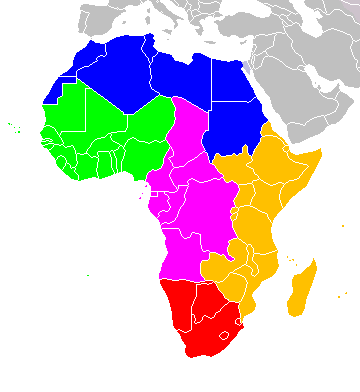
\includegraphics[width=0.75\textwidth]{Africa-regions.png}
	\caption{Africa: subregions as delineated by United Nations geographic classification scheme:
          \ccboxdsc{1.0,0.65,0.0} Eastern Africa, \ccboxdsc{1.0,0.0,1.0} Central Africa, \ccboxdsc{0.0,0.0,1.0} Northern Africa,
          \ccboxdsc{1.0,0.0,0.0} Southern Africa, \ccboxdsc{0.0,1.0,0.0} Western Africa. \emph{Wikipedia / CC BY-SA 3.0}}
	\label{fig:skycultures:AfricaRegions}
\end{figure}

\begin{figure}[htbp]
	\centering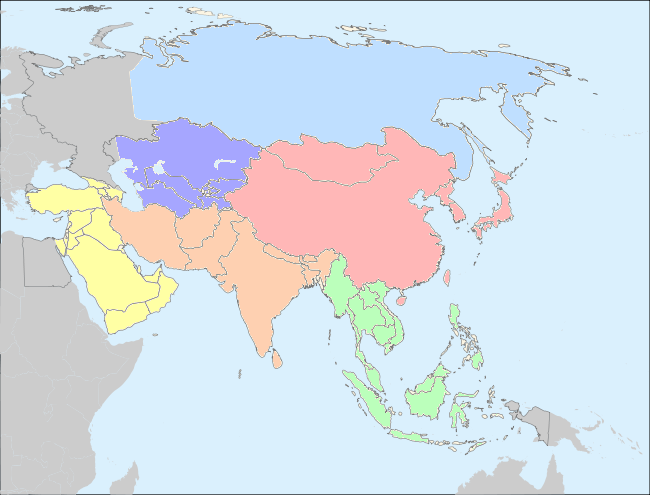
\includegraphics[width=0.75\textwidth]{Asia-regions.png}
	\caption{Asia: subregions as delineated by United Nations geographic classification scheme: \ccboxdsc{0.0,0.0,1.0} Central Asia,
          \ccboxdsc{1.0,0.0,0.0} Eastern Asia, \ccboxdsc{0.0,1.0,0.0} South-eastern Asia, \ccboxdsc{1.0,0.65,0.0} Southern Asia,
          \ccboxdsc{1.0,1.0,0.0} Western Asia, \ccboxdsc{0.75,0.88,1.0} Northern Asia. \emph{Wikipedia / CC BY-SA 3.0}}
	\label{fig:skycultures:AsiaRegions}
\end{figure}

\begin{figure}[htbp]
	\centering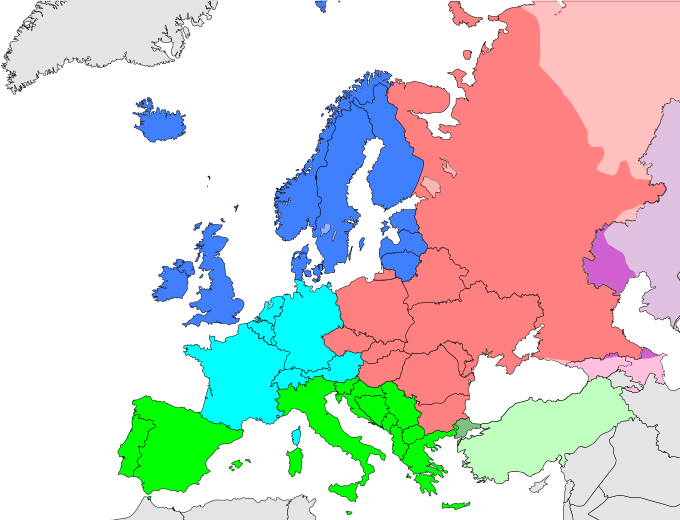
\includegraphics[width=0.75\textwidth]{Europe-regions.png}
	\caption{Europe: subregions as delineated by United Nations geographic classification scheme: \ccboxdsc{1.0,0.5,0.5} Eastern Europe,
          \ccboxdsc{0.25,0.5,1.0} Northern Europe, \ccboxdsc{0.0,1.0,0.0} Southern Europe, \ccboxdsc{0.0,1.0,1.0} Western Europe. \emph{Wikipedia / CC BY-SA 3.0}}
	\label{fig:skycultures:EuropeRegions}
\end{figure}

\begin{figure}[htbp]
	\centering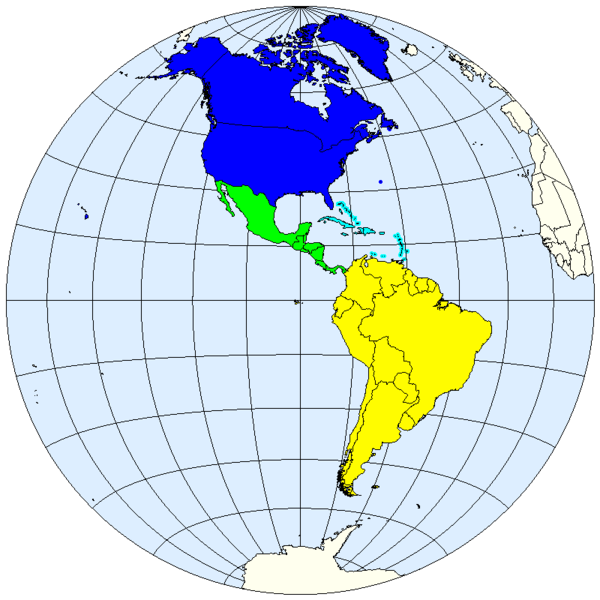
\includegraphics[width=0.7\textwidth]{Americas-regions.png}
	\caption{Americas: subregions as delineated by United Nations geographic classification scheme: \ccboxdsc{0.0,1.0,1.0} Caribbean,
          \ccboxdsc{0.0,1.0,0.0} Central America, \ccboxdsc{0.0,0.0,1.0} Northern America, \ccboxdsc{1.0,1.0,0.0} Southern America. \emph{Wikipedia / CC BY-SA 3.0}}
	\label{fig:skycultures:AmericasRegions}
\end{figure}

\begin{figure}[htbp]
	\centering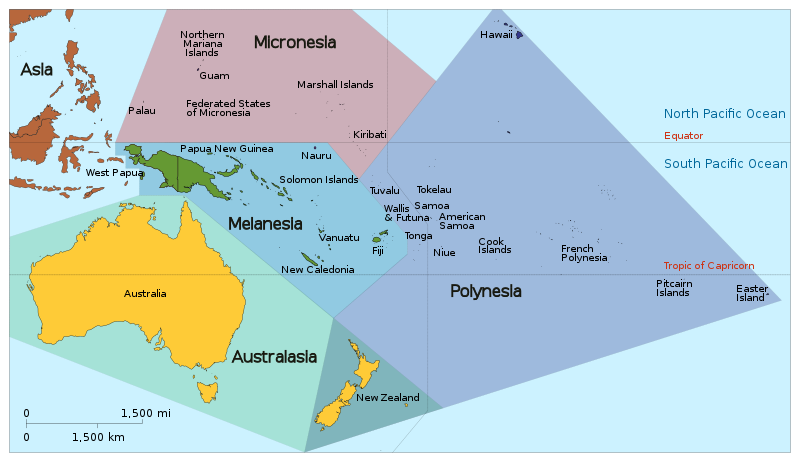
\includegraphics[width=\textwidth]{Oceania-regions.png}
	\caption{Oceania: subregions as delineated by United Nations geographic classification scheme: \ccboxdsc{1.0,0.8,0.2} Australasia, 
          \ccboxdsc{0.6,0.8,0.9} Melanesia, \ccboxdsc{0.8,0.7,0.7} Micronesia, \ccboxdsc{0.62,0.73,0.87} Polynesia. \emph{Wikipedia / CC BY-SA 3.0}}
	\label{fig:skycultures:OceaniaRegions}
\end{figure}



\subsection{Classification}
\label{SC:classification}

The tag ``classification'' allows describing the origin and intended use of this skyculture:
\begin{description}
  \item[personal] -- this is a personally developed sky culture which
    is not founded in published historical or ethnological research. Stellarium
    may include it when it is ``pretty enough'' without really
    approving its contents.
  \item[traditional] -- (default value) content represents ``common'' knowledge by
    several members of an ethnic community, and the sky culture has
    been developed by members of such community. Our ``Modern''
    sky culture is a key example: rooted in antiquity it has evolved for about 2500 years in what is now commonly known as ``western'' world,
    and modern astronomers use it.
  \item[ethnographic] -- provided by ethnographic researchers based on
    interviews of indigenous people.
  \item[historical] -- based on historical written sources from a
    (usually short) period of the past.
  \item[single] -- represents a single source like a historical atlas,
    or related publications of a single author.
  \item[comparative] -- special-purpose compositions \newFeature{0.21.2} of e.g.\ artwork
    from one and stick figures from another sky culture, and optionally
    asterisms as representations of a third. Or comparison of two
    stick figure sets in constellations and asterisms. These figures
    sometimes will appear not to fit together well. This may be
    intended, to explain and highlight just those differences! The
    description text must clearly explain and identify all sources and
    how these differences should be interpreted.
\end{description}


\subsection{Constellation boundaries}
\label{SC:boundaries}
\label{SC:edges}


In the late 18th century, when variable stars started to be catalogued by a code that included the star's constellation, 
a necessity arose to define which sky region belonged to which constellation. 
Atlases of this period showed curved boundaries between the constellations. 
Such boundaries are hard to describe by coordinates, though. The Uranographia Argentina proposed a different approach.
The boundaries were described by straight segments along great circles of equal right ascension and small circles of equal declination. 
The atlas used coordinates for epoch B1875.0. 
In 1930 the International Astronomical Union (IAU) ratified  this partition of the sky into the 88 constellations used by scientists and amateurs ever since.
When looking at these boundaries in J2000.0 coordinates, we can see they are no longer parallel to the J2000.0 coordinate grid, the deviation caused by precession. 

Partitions of the full sky into contiguous regions defined by edges between coordinate vertices defined in  
equatorial coordinates at a certain  epoch can be described in the following elements of the \file{index.json}:

\begin{jsonfile}[\scriptsize]
  "edges_type": "iau",
  "edges_source": "https://pbarbier.com/constellations/edges_18.txt",
  "edges_epoch": "B1875",
  "edges": [
    "001:002 M+ 22:52:00 +34:30:00 22:52:00 +52:30:00 AND LAC",
    "002:003 P+ 22:52:00 +52:30:00 23:20:00 +52:30:00 AND CAS",
    "004:005 P+ 23:20:00 +50:00:00 23:35:00 +50:00:00 AND CAS",
	...
	]
\end{jsonfile}


where
\begin{description}
\item[\jtag{edges\_type}] is optional and may contain the following values:
  \begin{description}
  \item[\texttt{"none"}] --- (default) designates that this culture doesn't have constellation boundaries, and any \texttt{edges} entry is ignored.
  \item[\texttt{"iau"}] --- use this value for variants of ``modern'' sky cultures to declare use of IAU boundaries.
  \item[\texttt{"own"}] --- used for cultures which have their own set of constellation boundaries.
  \end{description}

\item[\jtag{edges\_source}] is optional and only given for reference. It is not evaluated.

\item[\jtag{edges\_epoch}] describes the coordinate epoch. Allowed values: 
  \begin{description}
  \item[\texttt{"J2000"}] (default)
  \item[\texttt{"B1875"}] used for the edge list defining the IAU borders.
  \item[\texttt{"Byyyy.y"}] (a number with \texttt{B} prepended) Arbitrary epoch as Besselian year.
  \item[\texttt{"Jyyyy.y"}] (a number with \texttt{J} prepended) Arbitrary epoch as Julian year.
  \item[\texttt{"JDddddddd.ddd"}] (a number with \texttt{JD} prepended) Arbitrary epoch as Julian Day number.
  \item[\texttt{"ddddddd.ddd"}] (a pure number) Arbitrary epoch as Julian Day number.
  \end{description}
\end{description}

The lines in the array ``edges'' were taken from the given reference. The first component is ignored. 
The next element provides information whether the segment runs along a meridian (\texttt{M}, right ascension) or 
parallel (\texttt{P}, declination) circle in ascending \texttt{+} or descending \texttt{-} sense.  
Then it provides $\alpha_1$, $\delta_1$, $\alpha_2$, $\delta_2$ in sexagesimal numbers ($\alpha$ in HH:MM:SS, $\delta$ in DD:MM:SS format)
and the uppercased constellation abbreviations. As described in the original source file, 
Serpens has been split into \texttt{SER1} and \texttt{SER2}, these tags are treated both as \texttt{SER}.

These edges are used to define isolated boundaries for each constellation (for proper working of the \menu{Select single constellation} option). 



\subsection{Constellations}
\label{sec:skycultures:constellations}
\label{SC:constellations}

Constellations are coded as array of dictionaries:

\begin{jsonfile}[\scriptsize]
"constellations": [
    {
      "id": "CON modern Aql",
      "lines": [[98036, 97649, 97278], [97649, 95501, 97804], [99473, 97804], 
				[95501, 93747, 93244], [95501, 93805]],
      "image": {
        "file": "illustrations/aquila.png",
        "size": [512, 512],
        "anchors": [
          {"pos": [163, 232], "hip": 97649},
          {"pos": [385, 131], "hip": 93244},
          {"pos": [397, 397], "hip": 93805}
        ]
      },
      "common_name": {"english": "Aquila", "native": "Aquila"}
    }, ... 
], ...
\end{jsonfile}

where

\begin{description}
\item[\jtag{id}] A unique figure identifier, consisting of \texttt{CON} (for constellations), skyculture id, and a short label still unique within the skyculture.
                 For IAU-based skycultures, these short labels must be the IAU standard labels. For others, you can invent your own. It is not necessary to have exactly
                 3-letter keys, but they should act as mnemonic support, so numerical keys are not recommended:  
				 the short label is displayed when setting Constellation name style to ``short'' (s.~\ref{sec:gui:view:skyculture}). If you want to prevent
				 certain abbreviations from being displayed, let them start with a dot. See the effect in the \file{Modern (H.A.Rey)} sky culture: In
				 \menu{Abbreviated} mode, only the official abbreviations are displayed.
				 
				 
\item[\jtag{lines}] an array of arrays, each describing a polygon with star numbers. The star numbers are usually the Hipparcos (HIP) numbers. 
                    For very dim stars, the longer numbers from the Gaia DR3 catalog are acceptable, but they must be written as string.
					
					\emph{Single-star constellations}\newFeature{25.1}  or particular highlights can be described with just one star repeated in a two-element segment,
					the respective star will be encircled with a radius of \jtag{single\_star\_radius}.
					
					To describe \indexterm{dark constellations}\newFeature{25.2} formed from dust clouds in the Milky Way or other non-stellar items, 
					another variant can use coordinate lists and is technically an array of arrays of 2-part arrays of float numbers, 
					each pair being right ascension $\alpha$ (decimal hours) and declination $\delta$ (decimal degrees) in equinox J2000.0. 
\item[\jtag{single\_star\_radius}] (float, default 0.5)\newFeature{25.1}  radius of a circle (degrees) marking single-star segments in \jtag{lines}.
\item[\jtag{image}] Optional, see \ref{SC:image}
\item[\jtag{common\_name}] Dictionary of names. Required entries: \jtag{english}. Optional: \jtag{native}

	These names are used in the Constellation name style settings (s.~\ref{sec:gui:view:skyculture}): In \menu{Native} mode, the native element is shown. 
	Only with setting \menu{Translated}, the text translated from the english element is shown. If your sky culture is a variant of the \file{Modern}
	sky culture, please use the canonical Latin names, they have all been translated already.

	If your sky culture is not a variant of the generally known \file{Modern} (western)
	sky culture, please provide an English translation in addition to the name given in
	the native language. Else translators will not be able to translate
	the name. 

\item[\jtag{visibility}] (optional) special cases for rule-based visibility, e.g. seasonally changing aspects of figures. 
	Currently only a \jtag{months} rule has been defined. 
	Its ``payload'' is an array of two integers, start and end of visibility in months, e.g:

	\begin{jsonfile}
"visibility": {"months": [6, 3]},
	\end{jsonfile}
%
This specifies that the afflicted constellation is visible only from June to March. 
A second entry of the same constellation (with possibly different lines, artwork, or even name) 
that would be visible from April to May, would be specified as:
\begin{jsonfile}
"visibility": {"months": [4, 5]},
\end{jsonfile}
\end{description}







\iffalse REFERENCE?
You can \newFeature{0.19.2} add a reference comment after each
3-column entry. Just add a white-space, and then a comma-separated list
of numerical references to the books listed in \file{reference.fab}.
\fi



\subsubsection{Constellation Artwork}
\label{sec:skycultures:artwork}
\label{SC:image}

Constellation artwork is optional, but may give your sky culture the
final touch, if it requires artwork at all. E.g., H. A. Rey's variant
of the \file{Modern} sky culture deliberately does not contain artwork
other than his new set of stick figures.

Each constellation artwork is linked to 3 stars in its constellation. This
is programmed in the \jtag{image} dictionary. It contains entries
\begin{description}
\item[\jtag{file}] is the file name of your texture. All constellation artwork files should reside in a subdirectory \file{illustrations}. 
  For best efficiency it should be
  sized in a power of two, like $512\times512$, $1024\times2048$
  etc. Avoid dimensions larger than 2048, they are not supported on
  all systems. Use as little border in your textures as possible instead.
  You can distort images to better exploit the pixels,
  the texture will be stretched back. The background of the artwork
  image must be absolutely black.
  \item[\jtag{size}] Image size (width, height) in pixels. This size specified here, and not the real image size, is relevant for the \jtag{anchors} entry. 
  This may be important on very memory limited systems where you decide to downscale all textures.
  \item[\jtag{anchors}] An array of three similar dicts with
  \begin{description}
  \item[\jtag{pos}] pixel addresses [x, y] given from upper left corner (find those in any image editor)
  \item[\jtag{hip}] The star index as Hipparcos (HIP) number, given as integer. This may technically also be a Gaia DR3 number when given as string.
  \end{description}
\end{description}
%
In case the artwork is only available in a certain projection (e.g.,
an all-sky map), or is otherwise heavily distorted so that the match
is not satisfactory, you may have to re-project the image somehow. For
aligning, you should switch Stellarium to Stereographic projection for
optimal results.

You don't have to shutdown and restart Stellarium during
creation/matching, you can just press \key{Ctrl+\Alt+I} to reload.


\subsection{Asterisms and help rays}
\label{sec:skycultures:asterisms}
\label{SC:asterisms}

Sometimes auxiliary figures were created for easier orientation. Some part of a 
constellation was redefined into a figure in its own right, or  parts from different 
constellations were merged into one big figure --- e.g. ``Big Dipper'' as part of Ursa Major or the 
``Summer Triangle'' consisting of 3 stars from the constellations Cygnus, Lyra and Aquila. 
After the codification of the official 88 constellations by the IAU, those additional figures
are generally called \indexterm{asterisms}. \footnote{In a more generalized context when describing the sky of
  other cultures, the distinction may be less strict, and the term ``asterism'' may even be used 
  for the ``primary figures'' observed by those cultures.}

Other simple figures might be used as navigation and orientation helpers: the \indexterm{help rays}. 
As example to help in orientation in the sky the additional lines between constellations 
Ursa Major, Ursa Minor and Cassiopeia might be useful. The asterisms and help rays are listed in
\jtag{asterisms} which is similar to the \jtag{constellations} dict, but has no \jtag{figures} entry:

\begin{jsonfile}[\scriptsize]
"asterisms": [
    {
      "id": "AST modern HeG",
      "common_name": {"english": "Heavenly G", "references": [30,32]},
      "lines": [[21421, 24608, 36850, 37826, 37279, 32349, 24436, 25336, 27989]]
    }, ...
]
\end{jsonfile}

\begin{description}
\item[\jtag{id}] A unique asterism identifier, consisting of \texttt{AST} (for asterism), skyculture id, and a short label still unique within the skyculture.
                 It is not necessary to have exactly 3-letter keys, but they should act as mnemonic support, so numerical keys are not recommended:  
				 the short label is displayed when setting Constellation name style to ``short'' (s.~\ref{sec:gui:view:skyculture}). If you want to prevent
				 certain abbreviations from being displayed at all, let them start with a dot. 				 
\item[\jtag{common\_name}] Another dict with entries \jtag{english} (the translatable english name), 
				and an optional array \jtag{references} which lists from which sources (from \ref{SC:references}) this asterism was taken. 
				Collecting sources and giving such references is always a good idea. This entry may be used in later versions of Stellarium.
\item[\jtag{is\_ray\_helper}] (optional, default=\texttt{false}). 
                Set to \texttt{true} to declare this asterism as ``ray helper'' which is shown in a different color and without label. 
\item[\jtag{lines}] an array of arrays, each describing a polygon with integer star numbers. The star numbers are usually the Hipparcos (HIP) numbers. 
                    For the very dim stars of telescopic asterisms, the longer numbers from the Gaia DR3 catalog are acceptable, but they must be written as string.
					Another variant can use coordinate lists and is technically an array of arrays of 2-part arrays of float numbers, 
					each pair being right ascension $\alpha$ (decimal hours) and declination $\delta$ (decimal degrees) in equinox J2000.0. 

					\emph{Single-star asterisms} \newFeature{25.1} can be described with a two-element array that repeats the first entry (star or coordinate pair)
					-- the respective star/coordinate will be encircled with a radius of \jtag{single\_star\_radius}.
\item[\jtag{single\_star\_radius}] (float, default 0.5)\newFeature{25.1}  radius of a circle (degrees) marking single-star segments in \jtag{lines}.
\end{description}







\subsection{Names of Stars, Planets and Nonstellar Objects}
\label{sec:skycultures:starnames}
\label{SC:common_names}

Many cultures have defined their own names for stars, planets and even a few deep-sky objects bright enough to be seen with the unaided eye. 
The \jtag{common\_names} dict in a skyculture file \file{index.json} contains entries of arrays tagged with HIP catalog numbers or other names.

As example, we show a part of the Samoan skyculture\footnote{Sorry for the misspelling. Our typesetter does not like diacritics. The JSON file is correct!}:
\begin{jsonfile}[\scriptsize]
"common_names": {
    "HIP 32349": [{"english": "Gliding Star", "native": "Fetusolonu'u"}],
    "HIP 68702": [{"english": "Mea", "native": "Mea"}],
    "HIP 71683": [{"english": "Filo", "native": "Filo"}],
    "M45": [{"english": "Face of Li'i", "native": "MataliIi"}],
    "NGC2055": [{"english": "Pale Cloud", "native": "Aotea"}],
    "NGC292": [{"english": "Flying Cloud", "native": "Aolele"}],
    "NGC6093": [{"english": "Pae", "native": "Pae", "translators_comments": "Samoan Name"}],
    "NGC6121": [{"english": "Suga", "native": "Suga", "translators_comments": "Samoan Name"}],
    "NAME Earth": [{"english": "Earth", "native": "Lalolagi"}],
    "NAME Jupiter": [{"english": "Undying Mystery", 
	                  "native": "Tupualegase", 
					  "translators_comments": "Native name of Jupiter in Samoan"}],
    "NAME Mars": [{"english": "Reddish Face/Surface", 
	               "native": "Matamemea", 
				   "translators_comments": "Native name of Mars in Samoan"}],
    "NAME Mercury": [{"english": "Brownish", 
	                  "native": "Ta'elo", 
					  "translators_comments": "Native name of Mercury in Samoan"}],
    "NAME Moon": [{"english": "Moon", "native": "Masina"}],
    "NAME Saturn": [{"english": "Garland Star", "native": "Fetu'asoa", 
	                 "translators_comments": "Native name of Saturn in Samoan"}],
    "NAME Sun": [{"english": "Sun", "native": "La"}],
    "NAME Venus": [{"english": "Morning Star / Forbidden Radiance", 
					"native": "Tapu'itea", 
	                "translators_comments": "Native name of Venus in Samoan"}]
  }
\end{jsonfile}

\subsubsection{Star names}


The Keys for stars generally start with \jtag{HIP }. 
The associated array contains again dicts providing english spellings of the star names 
and \jtag{references} (optional but highly recommended) which indicates 
in which sources (see \ref{SC:references}) these star names or particular spellings occur.
Currently this has only documentary value for skyculture authors and researchers, but may become useful in later versions of Stellarium.
The \jtag{english} name will be translated. An additional \jtag{native} entry can be given, 
which is the culture-native version of the spelling 
(also in language-specific glyphs when available in UTF8 and the current font) and will never be translated but can be shown on screen if so configured.


\begin{jsonfile}[\scriptsize]
"common_names": {
    "HIP 677": [{"english": "Alpheratz", "references": [1,2,5,6,11,12,37]},
                {"english": "Sirrah", "references": [23,37]}],
    "HIP 746": [{"english": "Caph", "references": [1,2,6,11,12,23,37]},
                {"english": "Al Sanam al Nakah", "references": [37]}],
	... }
\end{jsonfile}

When there is more than one name for a star, the first in the list is used as screen label. 
% TODO
% Alternatively, one of the dicts can have an optional tag \jtag{label}\texttt{: true}, in which case this string (or translation) 
% is used as screen label if the star name setting is set to short. \newFeature{25.2}   
% This can be used for more technical labels (star list numbers).


\subsubsection{Planet Names}
\label{sec:skycultures:planetnames}

The  \jtag{common\_names} dict can also contain native names of the planets. 
For these, the JSON key is formed from \jtag{NAME }, a space and the English name of the planet. 
The value vector provides dicts which include 
\begin{description}
\item[\jtag{english}] (the translatable name), 
\item[\jtag{native}] (optional) native spelling, may be in native glyphs when supported by UTF8, 
\item[\jtag{transliteration}] (optional) Native name in European glyphs, if needed.
\item[\jtag{translators\_comments}] (optional) comments to be shown to translators on Transifex, 
\item[\jtag{references}] (optional) the sources for these names where applicable.
\end{description}

In earlier versions it was recommended to combine the native name with an English translation. 
In the new format here we should keep them separate, and the actual screen label can be combined from available components on the fly.\newFeature{25.2}
However, for languages with non-European glyphs please include a transliteration as pronounciation aid to the \jtag{english} string.
% TODO: Shall we add an optional \jtag{transliteration} tag which could itself again be translatable?



\subsection{Deep-Sky Objects Names}
\label{sec:skycultures:dsonames}

\jtag{common\_names} can also contain native names for
deep-sky objects (DSO). The content  of the dicts is similar to the 
format for planet names above. % (see \ref{sec:skycultures:planetnames}).
Known tags are 
\begin{description}
\item[\jtag{english}] English meaning
\item[\jtag{native}] (optional) Native name. May be in native glyphs when supported in UTF8.
\item[\jtag{transliteration}] (optional) Native name in European glyphs, if needed.
\item[\jtag{translators\_comments}] (optional) English explanations that help in translation. Not displayed in the program.
\item[\jtag{references}]  (optional) the sources for these names where applicable
\end{description}



\section{The Skyculture Converter}
\label{ch:SkyCultures:converter}

Many sky cultures have been created and maintained outside of Stellarium. They follow the old format, which is no longer supported since Stellarium version 25.1. To ease the transition we've developed a converter tool. It is a console application that takes a path to the old-format sky culture directory, and a path where to put the converted sky culture. Example command to run it:

\begin{commands}
skyculture-converter c:\samoan.old c:\samoan
\end{commands}

While the converter tries hard to convert the description text from HTML to Markdown adding some sections from other parts of the sky culture, the conversion may not be ideal. Formerly the description was completely free in structure, while now there are some requirements on it, so the text may need some editing to conform.

If you have gettext translation files (the ones whose names are in the form \texttt{locale-name.po}) for the names of stars, constellations etc., you can pass the path to the directory that contains them as an optional third argument to the converter.

Additionally, there are some options that you can use to control the conversion:

\begin{description}
\item[\texttt{-\/-footnotes-to-references}] Convert footnotes in a particular form to references. Such footnotes are expected to be in the form of
\begin{htmlbit}
<p id="footnote-9">This is a footnote</p>
\end{htmlbit}
while the references to them are expected to be in the form of
\begin{htmlbit}
<sup><a href="#footnote-9">[9]</a></sup>
\end{htmlbit}
\item[\texttt{-\/-untrans-names-are-native}] Put the names that in \texttt{star\_names.fab} or in \texttt{dso\_names.fab} are denoted without an underscore into the \texttt{native} section of the name, rather than \texttt{english}. For example, with this option \texttt{32349|("Fētūsolonuʻu")} would be treated as a native name, while \texttt{32349|\_("Gliding Star")} would be treated as an English one.
\item[\texttt{-\/-native-locale LOCALE}] Some sky cultures have, in addition to \texttt{star\_names.fab} or \texttt{dso\_names.fab}, localized versions of them, like e.g. \texttt{star\_names.zh\_CN.fab}, that were never actually used but do contain useful information. If you pass the locale (\texttt{zh\_CN} in this example) as the \texttt{LOCALE} parameter, these names will be read and put into the \texttt{native} section of the corresponding JSON entry. Note that the order of stars/DSOs in the normal and localized files much be the same, otherwise there's no way to match the names.
\item[\texttt{-\/-translated-md}] To check the look of the translated description texts you can use this option. The output directory will contain, in addition to \texttt{description.md}, files named like \texttt{description.es\_419.DO\_NOT\_COMMIT.md}, with the ``DO NOT COMMIT'' part reminding you that they are not a part of the sky culture.
\end{description}

\section{Publish Your Work}
\label{sec:skyculture:publish}

If you are willing to let other users enjoy the result of your hard
work (and we certainly hope you do!), when you are done, please write
a note in the Forum or at GitHub. We will decide about acceptability
and classification, or may ask for better descriptions for the
benefit of our users.

Please put the imagery and text
under some compatible open-source license (see ~\ref{SC:license}).
Else the sky culture cannot be hosted by us.
While we cannot be held responsible for legal problems, it seems that
CC BY 4.0 International\footnote{\url{https://creativecommons.org/licenses/by/4.0/}} or
CC BY-SA 4.0 International\footnote{\url{https://creativecommons.org/licenses/by-sa/4.0/}}
licenses are best suited. See notes in section~\ref{sec:skycultures:licenses} above. 


%%% Local Variables: 
%%% mode: latex
%%% TeX-master: "guide"
%%% End: 

